\section{Exploratory Data Analysis}

The goal of exploratory data analysis (EDA) is to understand the dataset and its features. This process involves examining the data, identifying patterns, and summarizing the main characteristics of the dataset. We first provide a detailed analysis of the features and their distributions, describe the correlations between features, and justify our lack of dimensionality reduction.

\subsection{Feature Distributions}
For each feature, we created and examined either a histogram and boxplot (for numerical features) or a bar chart (for categorical features). An example plot for the distribution of age is given in Fig.~\ref{agedist}. For each feature, we also recorded descriptive statistics and noted whether there were any outliers, missing values, or rare categories.

\begin{figure}[htbp]
    \centerline{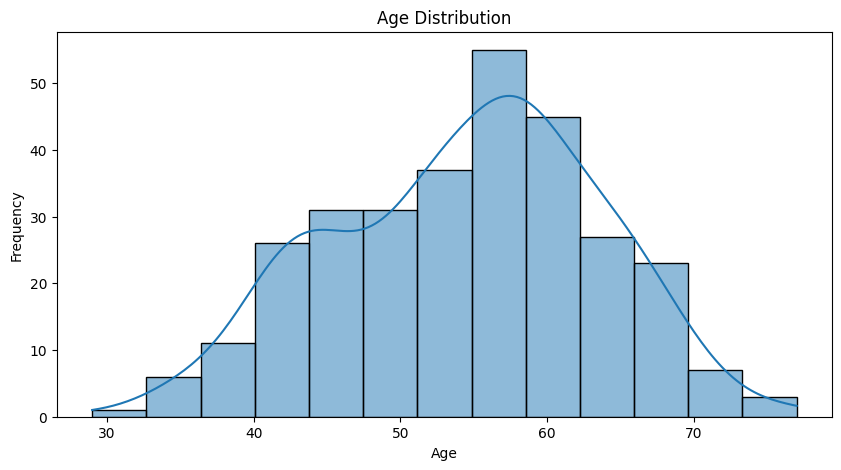
\includegraphics[width=0.7\columnwidth]{img/agedist.png}}
    \caption{Distribution of Age.}\label{agedist}
\end{figure}

From this analysis, we determined that most numerical features are approximately normally distributed, with the exception of ``ST Depression Induced by Exercise on an ECG'' which is heavily skewed right. This feature also contained zero values, but this is expected given the nature of the test \cite{katheria2021stdepression}. All numerical features except for ``Age'' contain outliers as computed with the 1.5 IQR rule, with ``Resting Blood Pressure'' containing the most. However, since there are not very many outliers (<2\% of the dataset for each feature) and outliers are not extreme, we decided to keep them in the dataset. We also found that the feature ``Number of Major Vessels Colored by Flourosopy'' contains four missing values (approximately 1\% of the dataset). Since the this feature is numerical and the number of missing values is realtively small, we decided to impute the missing values with the mean of the feature.
We determined that the majority of categorical features have imbalanced classes. Notably, only 32\% of the patients in the dataset are female, which may affect how well the model generalizes to the general population.

\subsection{Feature Correlations}
To determine the relationship between the features in the dataset, we performed a correlation analysis on the data. For each pair of numerical features, we created a scatter plot. We also created a correlation heatmap of the data, shown in Fig. ~\ref{featureheatmap}. Based on the correlation heatmap, we determined that no two features are especially correlated (other than ``oldpeak'' representing ST-segment depression on an ECG during exercise, and ``slope'' representing ST/HR slope).

\begin{figure}[htbp]
    \centerline{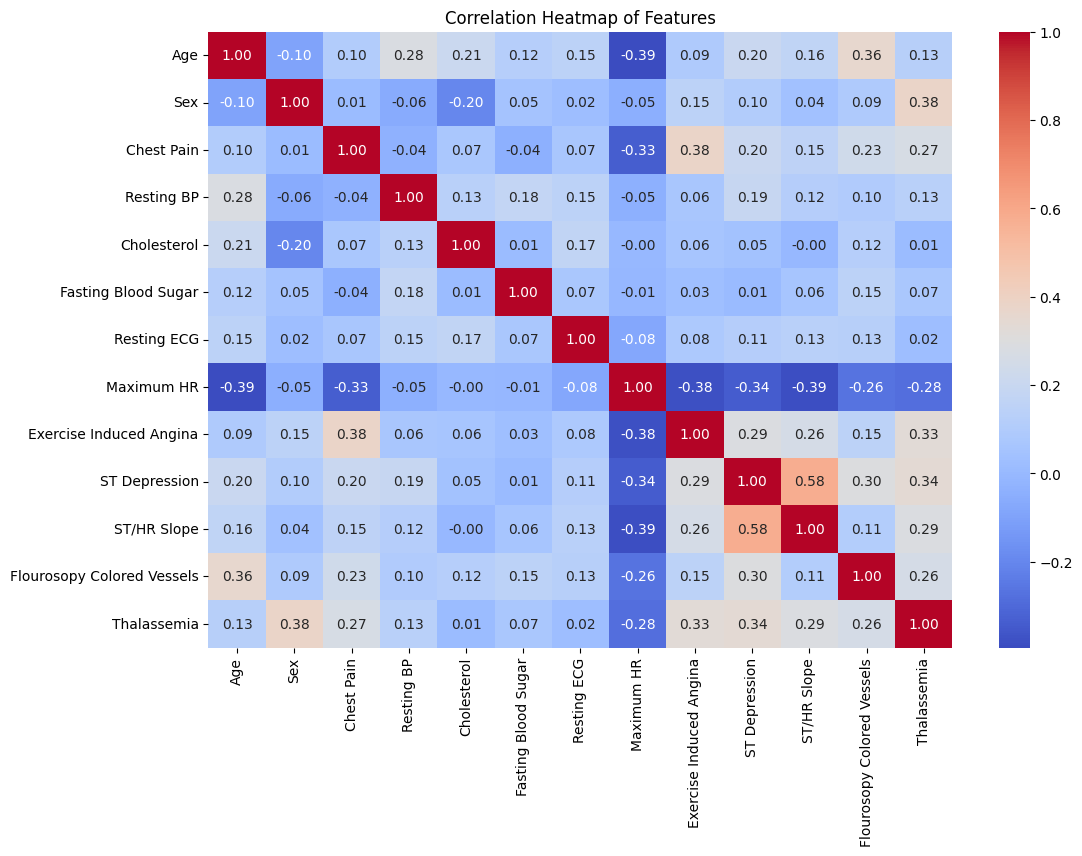
\includegraphics[width=0.7\columnwidth]{img/featureheatmap.png}}
    \caption{Feature Correlation Heatmap.}\label{featureheatmap}
\end{figure}

\subsection{Dimensionality Reduction}
We did not perform any dimensionality reduction on the dataset. The dataset contains only 13 features, which is tractable for all the models we chose. We also did not find any features that were highly correlated with each other, so we did not need to remove any features on the basis of correlation. To corroborate our lack of dimensionality reduction, we conducted a principal component analysis (PCA) on the dataset to determine if there were any features that could be removed on the basis of a very low explained variance. We found that all 13 principal components carried a non-insignificant amount of variance (>2\% for all components), shown in Fig.~\ref{pca}. Due to the low number of features and the lack of correlation between features, we decided to keep all features in the dataset.

\begin{figure}[htbp]
    \centerline{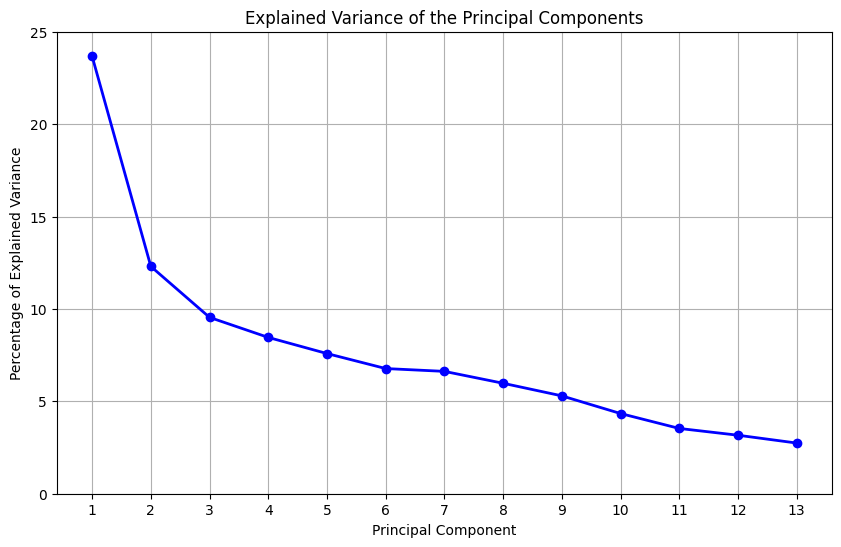
\includegraphics[width=0.7\columnwidth]{img/pca.png}}
    \caption{Explained Variance of Principal Components.}\label{pca}
\end{figure}